
\begin{frame}
  \frametitle{Le RCPSP}
 \vspace{0.4cm}
 \textbf{Inputs : }
 \vspace{0.4cm}
  \begin{itemize}
  \item a set ${\cal A}=\{1,\dots ,n\}$ of non-preemptive tasks
    \vspace{0.4cm}
  \item a set ${\cal R}=\{1,\dots ,m\}$ of cumulative and renewable resources available in quantity $B_k$
      \vspace{0.4cm}
  \item<2-> for each task:
    \begin{columns}
      \hfill
      \begin{column}{0.5\linewidth}
        \begin{itemize}
          \vspace{-0.6cm}
        \item<2-> \footnotesize  a processing time $p_i$
          \vspace{0.25cm}
        \item<3-> \footnotesize a resource consumption $b_{ik}$ on each
          resource $k \in {\cal R}$ 
          \vspace{0.25cm}
        \item<4-> \footnotesize a set of predecessors $prec_i $
          \vspace{0.25cm}
        \end{itemize}
      \end{column}
      \hfill
      \begin{column}{0.4\linewidth}
        \centering
          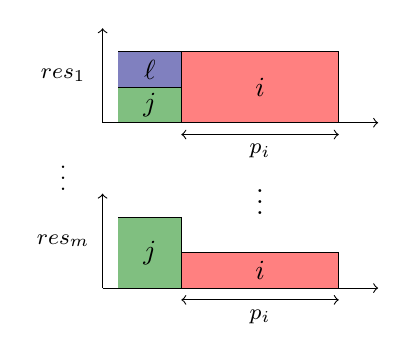
\begin{tikzpicture}
  [yscale=0.3]
  \node[label={[shift={(-0.4,-0.5)}]}] (O) at (0,0) {};
  \draw[fill=red!50] (1,0) rectangle (3,3)   node[midway] {$i$};
  
  \onslide<2-3>{
    \draw[<->] (1,-0.5) -- (3,-0.5) node[midway,below] {\footnotesize $p_i$};
  }
  \onslide<3>{
    \draw[<->] (0.8,0) -- (0.8,3) node[midway,left] {\footnotesize $b_{i1}$};
  }
  
  \draw[->] (O.center) -- (0,4);
  \draw[->] (O.center) -- (3.5,0);


  \onslide<3->{
  \node at (2,-3) {$\vdots$};

  \draw[fill=red!50] (1,-7)rectangle (3,-5.5) node[midway] {$i$};
  
  \onslide<3>{
    \draw[<->] (1,-7.5) -- (3,-7.5) node[midway,below] {\footnotesize $p_i$};
  }
  \onslide<3>{
    \draw[<->] (0.8,-7) -- (0.8,-5.5) node[midway,left]
    {\footnotesize $b_{im}$};
  }
  
  \node at (-0.5,2) {\footnotesize $res_1$};
  \node at (-0.5,-5) {\footnotesize $res_m$};
  \node at (-0.5,-2) {\footnotesize $\vdots$};

  \draw[->] (0,-7) -- (0,-3);
  \draw[->] (0,-7) -- (3.5,-7);
}
\onslide<4->{
  \fill[color=green!50!black!50] (0.2,0) rectangle (1,1.5);
  \draw (0.2,0) -- (1,0) -- (1,1.5) -- (0.2,1.5) ;
  \path (0.2,0.75) -- (1,0.75) node[midway] {$j$};

  \fill[color=blue!50!black!50] (0.2,1.5) rectangle (1,3);
  \draw (0.2,1.5) -- (1,1.5) -- (1,3) -- (0.2,3) ;
  \path (0.2,2.25) -- (1,2.25) node[midway] {$\ell$};


  \fill[color=green!50!black!50] (0.2,-7) rectangle (1,-4);
  \draw (0.2,-7) -- (1,-7) -- (1,-4) -- (0.2,-4) ;
  \path (0.2,-5.5) -- (1,-5.5) node[midway] {$j$};
}
\end{tikzpicture}

      \end{column} 
      \hfill
    \end{columns}
  \end{itemize} 
\end{frame}


\begin{frame}
  \frametitle{Context}
  \begin{itemize}
  \item Time-indexed model more efficient {\small (relatively stronger relaxation)}
\pause
    \vfill
  \item But:
    \begin{itemize}
    \item  model size depends on planning horizon 
      
      $\longrightarrow $ for large planning horizon event-based model can be more
      efficient (RCPSP:~{\color{gray!50!black!70}\it [Koné et al.,
        2011]} )
      \vfill
\pause
    \item  if only non-integer solutions
      
      $\longrightarrow$ time-indexed model can lead to
      infeasible/sub-optimal solution
      (CECSP:~{\color{gray!50!black!70}\it [Nattaf et al., 2015]} )
    \end{itemize}
  \end{itemize}
\vfill
\pause
{\bf Goal: Tightened Event-based model (On/off)} 
\end{frame}

\begin{frame}{Event-based model }
  \vfill
  \begin{itemize}
  \item Start/End and On/Off model have a commun subset of constraints
    \pause
    \vfill
  \item Study of the polyhedron defined by these constraints
    \pause
    \vfill
  \item Collaboration with Tamas Kis 
  \end{itemize} 
  \vfill
\end{frame}

\begin{frame}{Event-based model }
  \vfill 
  \begin{tabularx}{\textwidth}{XclXc}
    \multicolumn{2}{l}{\bf Start/End Model} & &
    \multicolumn{2}{l}{\bf On/Off Model}\\[2mm]
    \textcolor<1>{blue!80!black!80}{ \scriptsize $t_e \le t_{e+1} $}&
    \textcolor<1>{blue!80!black!80}{ \scriptsize $\forall e$ }&
    &
    \textcolor<1>{blue!80!black!80}{ \scriptsize  $t_e \le t_{e+1}$ }& 
    \textcolor<1>{blue!80!black!80}{ \scriptsize $\forall e$}\\[2mm]
    
\pause
    \textcolor<2>{blue!80!black!80}{ \scriptsize $x_{ie}est_i \le t_e$ }&
    \textcolor<2>{blue!80!black!80}{ \scriptsize $ \forall e,i $ }&
    &
    \textcolor<2>{blue!80!black!80}{ \scriptsize $est_iz_{ie}\le t_e
      $} & 
    \textcolor<2>{blue!80!black!80}{ \scriptsize $\forall e, i $}\\[2mm]

    \textcolor<2>{blue!80!black!80}{ \scriptsize $ t_e \le x_{ie}lst_i +
    (1-x_{ie})D_{max}$ }& 
  \textcolor<2>{blue!80!black!80}{ \scriptsize $ \forall e,i $ }&
  & 
  \textcolor<2>{blue!80!black!80}{ \scriptsize $t_e \le
    lst_i(z_{ie}-z_{ie-1})+(1-(z_{ie}-z_{ie-1}))D_{max}$ }&
    \textcolor<2>{blue!80!black!80}{ \scriptsize $ \forall e,i$}\\[2mm]

\pause
    \textcolor<3>{blue!80!black!80}{ \scriptsize $let_iy_{ie}
    +(1-y_{ie})D_{max} \ge t_e $} & 
  \textcolor<3>{blue!80!black!80}{ \scriptsize $\forall e,i$}& 
  &
  \textcolor<3>{blue!80!black!80}{ \scriptsize  $eet_i(z_{ie-1}-z_{ie})\le t_e$}
    & \textcolor<3>{blue!80!black!80}{ \scriptsize $\forall e, i $}\\[2mm]

    \textcolor<3>{blue!80!black!80}{ \scriptsize $t_e \ge eet_iy_{ie} $ }&
    \textcolor<3>{blue!80!black!80}{ \scriptsize $\forall e,i$}&
    &
      \textcolor<3>{blue!80!black!80}{ \scriptsize
    $t_e \le let_i(z_{ie-1}-z_{ie})+(1-(z_{ie-1}-z_{ie}))D_{max}$ }&
    \textcolor<3>{blue!80!black!80}{ \scriptsize $\forall e, i $}\\[2mm]

\pause
    \textcolor<4>{blue!80!black!80}{ \scriptsize $\sum_{e\in {\cal E}}
    x_{ie} =1 $}& \textcolor<4>{blue!80!black!80}{ \scriptsize$ \forall i $}&
  & \textcolor<4>{blue!80!black!80}{
    \scriptsize$\sum_{e \in {\cal E}} z_{ie} \ge 1$}&
    \textcolor<4>{blue!80!black!80}{ \scriptsize$ \forall i $} \\[2mm]

    \textcolor<4>{blue!80!black!80}{ \scriptsize $\sum_{e\in {\cal E}}
    y_{ie} =1 $}& \textcolor<4>{blue!80!black!80}{ \scriptsize$ \forall i$ }&
    \textcolor<4>{blue!80!black!80}{ }& \textcolor<4>{blue!80!black!80}{ \scriptsize
    $\sum_{e'=1}^{e} z_{ie'} \le e(1-(z_{ie}-z_{ie-1}))$ }&
    \textcolor<4>{blue!80!black!80}{ \scriptsize$ \forall e,i$}\\[2mm]

    & \textcolor<4>{blue!80!black!80}{ }& \textcolor<4>{blue!80!black!80}{} &
    \textcolor<4>{blue!80!black!80}{ \scriptsize $\sum_{e'=e}^{2n} z_{ie'} \le
    (2n-e)(1+(z_{ie}-z_{ie-1})) $}& \textcolor<4>{blue!80!black!80}{
    \scriptsize$ \forall e,i$}
  \end{tabularx}
  \vfill
\end{frame}

\begin{frame}{Work done during the thesis}
  \vfill
  \begin{itemize}
  \item Start/End model have stronger relaxations than the On/Off
    model ( $z_{ie} = \sum_{f=1}^e x_{if} - \sum_{f=1}^e y_{if}$)
    \vfill 
\pause
  \item Upper bound on the distance between to event
    \vfill
\pause
  \item Upper bound on the date of each event
    \vfill
\pause
  \item Knapsack inequalities
    \vfill
\pause
  \item Description of the "On/Off Polyhedron"
  \end{itemize}
  \vfill
\end{frame}

\subsection{Valid inequalities}
\begin{frame}
  \frametitle{Maximum separation between events}
  \begin{itemize}
  \item {\bf Goal: } upper bound on the value of $t_{e+1}-t_{e}$
    \vspace{0.3cm}
  \item<2-> Time window of each task start and/or end time
    \vspace{0.3cm}
  \item<6-> An event must occur in each of these time windows
    \vspace{0.3cm}
  \item<11-> two consecutive events in the union of two consecutive time windows
  \end{itemize}
  \vfill
  \onslide<3->{
    \begin{center} 
      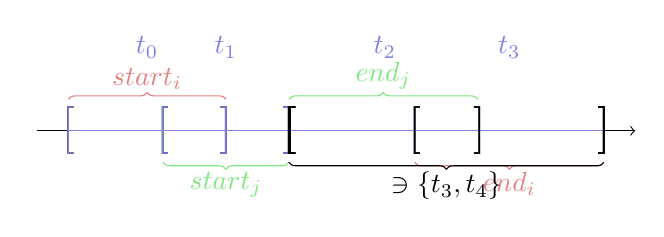
\begin{tikzpicture}
        [decoration={brace},scale=0.4]
        \node (O) at (0,0) {}; 
        \draw[->] (0,0) -- (19,0);

        \onslide<4-5>{
          \path (1,0) node[color=red!80!black!50] {\LARGE [} --
          +(0:5cm)node[color=red!80!black!50] {\LARGE ]};
          \path[green!80!black!50](4,0) node {\LARGE [} -- +(0:4cm)
          node {\LARGE ]};
          \path[green!80!black!50] (8.05,0) node {\LARGE [}  --
          +(0:6cm) node {\LARGE ]}  ;
          \path (12,0) node[color=red!80!black!50] {\LARGE [} --
          +(0:6cm) node[color=red!80!black!50] {\LARGE ]} ; 
        }
        
        \onslide<4>{
          \draw [decorate,color=red!80!black!50] (1,1) -- +(0:5cm)
          node[midway,above]{$start_i$}; 
          \draw [decorate,color=red!80!black!50] (18,-1) -- +(0:-6cm)
          node[midway,below] {$end_i$};
        }
        
        \onslide<5>{
          \draw [decorate,green!80!black!50] (8,-1) -- +(0:-4cm)
          node[midway,below] {$start_j$};
          \draw [decorate,green!80!black!50] (8,1) -- +(0:6cm)
          node[midway,above] {$end_j$};
        }
        
        \onslide<6-9>{
          \path (1,0) node {\LARGE [} --
          +(0:5cm)node {\LARGE ]};
          \path(4,0) node {\LARGE [} -- +(0:4cm)
          node {\LARGE ]};
          \path (8.05,0) node {\LARGE [}  --
          +(0:6cm) node {\LARGE ]}  ;
          \path (12,0) node {\LARGE [} --
          +(0:6cm) node {\LARGE ]} ; 
        }

        \onslide<6>{
            \path[blue!80!black!50,draw] (1,0) node {\LARGE [} -- +(0:5cm)node
            {\LARGE ]} node[midway,above=0.8cm] {$t_0$};
          }
          \onslide<7>  {
            \path[blue!80!black!50,draw](4,0) node {\LARGE [} --
            +(0:4cm) node {\LARGE ]} node[midway,above=0.8cm] {$t_1$}; 
          }
          
          \onslide<8>{   
            \path[blue!80!black!50,draw] (8.05,0) node {\LARGE [}  --
            +(0:6cm) node {\LARGE ]}  node[midway,above=0.8cm] {$t_2$};
          }
          
        \onslide<9>{
          \path[blue!80!black!50,draw] (12,0) node {\LARGE [} --
          +(0:6cm) node {\LARGE ]} node[midway,above=0.8cm] {$t_3$};
        }
        
        \onslide<10>{
          \path (12,0) node {\LARGE [}  --
          +(0:6cm) node {\LARGE ]}  ;
        \path (8.05,0) node {\LARGE [}  --
        +(0:6cm) node {\LARGE ]}  ;
    }
        \onslide<11>{
          \path (12,0) --
          +(0:6cm) node {\LARGE ]}  ;
          \path (8.05,0) node {\LARGE [}  --
          +(0:6cm)  ;
    }
    
    \onslide<12>{
  \path (8,0) node {\LARGE [} --
        +(0:10cm) node {\LARGE ]}  ;
        \draw [decorate] (18,-1) -- +(0:-10cm)
        node[midway,below] {$\ni \{t_3,t_{4}\}$};
      }
    \end{tikzpicture}
  \end{center}
}
\end{frame}

\begin{frame}
  \frametitle{Maximum separation between events}
  \begin{itemize}
  \item Order the time-window intervals according to:
    \[ [a,b] \le [c,d]
      \Leftrightarrow a < c \lor \left( a=c \land b \le d\right)\]
    \vfill
\pause
  \item Then we have:
    \[t_{e+1}-t_e  \le   |tw_e \cup tw_{e+1}|    \]
\pause
\begin{flushright}
    \textcolor{black!70}{\scriptsize in fact: $t_{e+1}-t_e  \le
      \overline{tw_e \cup tw_{e+1}} - \underline{tw_e \cup tw_{e+1}}
      $}
\end{flushright}
\pause
\vfill
  \item We can use it as:
\begin{itemize}
\vspace{0.2cm}
\item additional constraints of the model
\item an upper bound on $t_{e+1}-t_e$ in any constraints using a worst one
\end{itemize}
  \end{itemize}
\end{frame}

\begin{frame}
  \frametitle{Maximum time for an event}
  \begin{itemize}
  \item {\bf Goal: } upper bound on the value of $t_{e}$
    \vspace{0.4cm}
  \item<2-> upper bound of each task start and/or end time
    \vspace{0.4cm}
  \item<5-> an event must occur before each of these upper bounds
    \vspace{0.4cm}
  \end{itemize}
  \vfill
  \onslide<3->{
    \begin{center} 
      \begin{tikzpicture}
        [decoration={brace},scale=0.4]
        \node (O) at (0,0) {}; 
        
        \draw[->] (0,0) -- (19,0);
        \onslide<3>{
          \draw (1,0) node {\LARGE [} -- +(0:5cm)node {\LARGE ]}; 
        
        \draw(4,0) node {\LARGE [} -- +(0:4cm) node {\LARGE ]} ;
   
        \draw (8.05,0) node {\LARGE [}  --
        +(0:6cm) node {\LARGE ]}  ;
                \draw (12,0) node {\LARGE [} --
        +(0:6cm) node {\LARGE ]}  ;}
      \onslide<4>{
  
        \draw (1,0) node {} -- +(0:5cm)node {\LARGE ]}; 
        
        \draw(4,0) node {} -- +(0:4cm) node {\LARGE ]} ;
   
        \draw (8.05,0) node {}  --
        +(0:6cm) node {\LARGE ]}  ;
                \draw (12,0) node {} --
        +(0:6cm) node {\LARGE ]}  ;}
      \onslide<5>{
          \draw[color=blue!80!black!50] (0,0) node {} -- +(0:6cm)node {\LARGE ]}
          node[left,above=0.8cm] {$t_0$}; 
          \draw (8,0) node {\LARGE ]} ;
          \draw (8.05,0) node {}  -- +(0:6cm) node {\LARGE ]}  ;
          \draw (12,0) node {} -- +(0:6cm) node {\LARGE ]}  ;}
      
        \onslide<6>{
          \draw (6,0) node  {\LARGE ]}; 
          \draw[color=blue!80!black!50](0,0) -- (8,0) node {\LARGE ]} node[left,above=0.8cm] {$t_1$};
          \draw (8.05,0) node {}  --  +(0:6cm) node {\LARGE ]}  ;
          \draw (12,0) node {} --  +(0:6cm) node {\LARGE ]}  ;}
      
        \onslide<7>{
          \draw (6,0) node {\LARGE ]}; 
          \draw (8,0) node {\LARGE ]} ;
          \draw[color=blue!80!black!50] (0,0) node {}  -- (14,0) node {\LARGE ]} node[left,above=0.8cm] {$t_2$} ;
          \draw (18,0)node {\LARGE ]}  ;}
        
        \onslide<8>{
          \draw (6,0) node {\LARGE ]}; 
          \draw(8,0) node {\LARGE ]} ;
          \draw (14,0) node {\LARGE ]}  ;
          \draw[color=blue!80!black!50] (0,0) node {} -- (18,0) node {\LARGE ]}
          node[left,above=0.8cm] {$t_3$};} 
      
      \end{tikzpicture}
    \end{center}
  }
\end{frame}


\begin{frame}
  \frametitle{Maximum time for an event}
  \begin{itemize}
  \item Order the time-window interval upper bounds ${\cal UP}$ in
    increasing order 
\vfill
\pause
  \item Then we have:
\[t_e \le  {\cal UP}_e\]
\vfill
\pause
\item We can use it as:
\begin{itemize}
  \vspace{0.2cm}
\item additional constraints of the model
\item an upper bound on $t_{e+1}-t_e$ in any constraints using a worst one
\end{itemize}
  \end{itemize}
\end{frame}

\subsection{Polyhedral results}


\begin{frame}
  \frametitle{$Z_i$-polyhedron}
\vspace{0.5cm}
  \onslide<1->{$\rightarrow$ Minimal set of inequalities defining the
    {\it ``$Z_i$-polyhedron''}.}
\vspace{0.6cm}
    \onslide<2-> {  \begin{block}{$Z_i$-polyhedron}
 form of $z_i \in \{0,1\}^{|{\cal E}|}$ solution? \hspace{2.5cm}
      {\scriptsize (${\cal E}=$event set)}}
    \vspace{0.4cm}

\onslide<4->{$\Rightarrow$ vector with consecutive-one property  and at least
    one $1$
    \begin{center}
      {\small e.g. $(0,0,1,1,1,0),\ (1,1,1,0,0,0),\ \dots$}
    \end{center}}
\onslide<5->{     
    \[Z_i= conv\{z_i \in \{0,1\}^{|{\cal E}|} | z_i \text{ of the
        form } (0^*\, 1\, 1^*\, 0^*)\} \] }
\vspace{-0.2cm}
  \end{block}
  \onslide<3->{\textcolor{black!70}{ \small\[z_{ie}=\left\{
        \begin{array}{ll}
          1 & \text{if task $i$ is in process between $t_e$ and $t_{e+1}$}\\
          0 & \text{otherwise}
        \end{array}
      \right.
    \]}}
\end{frame}
  
\begin{frame}
\frametitle{Non-preemptive inequalities}
  \begin{block}{Non-preemptive inequalities}
    \[\sum_{e_k \in S} (-1)^kz _{ie_k} \leq 1\]
    where $S = \{e_0,e_1,\ldots,e_{2\ell}\}$ is a subset of 
    ${\cal E}$ of odd cardinality.
  \end{block}

    \vspace{0.6cm}
  \begin{itemize}
  \item<2-> e.g. with $S=\{3,6,11,13,18\}$
    \[ z_{i3} - z_{i6} + z_{i11}-z_{i13} +z_{i18} \le
      1 \]
\vfill
  \item<3-> If $|S|=3$ then $ z_{ie}-z_{if}+z_{ig} \le 1$ enforces
    $z_{if}$ to be $1$ for all $e<f<g$ s.t. $z_{ie}=z_{ig}=1$ 
  \end{itemize}

\end{frame}

\begin{frame}
  \frametitle{$Z_i$-polyhedron}
  \[ZP_i=\{ z_i \in [0,1]^{\cal E} | z_i\text{ satisfies
      non-preemptive inequalities and } \eqref{eq1}\}\] 
  \begin{equation}
    \text{ with }  \sum_{e \in \cal E} z_{ie} \ge 1 \quad \forall i \in \cal A  
    \label{eq1}  
  \end{equation}
  \pause
  \begin{block}{Theorem}
    \[ZP_i=Z_i\]
  \end{block}
  \vspace{0.5cm}
  \onslide<3->{\begin{itemize}
    \item[\bf Proof] {\small $\bullet$ use Farkas lemma to define inequalities
        over which $z \in Z_i$}
      \vspace{0.1cm}
    \item[ ] {\small $\bullet$ show that this inequalites are in bijection with the one
        \invisible{$\bullet$}~defining $ZP_i$}
    \end{itemize}
  }
  \vspace{0.2cm}
  \onslide<2->{\textcolor{black!70}{\small \[Z_i= conv\{z_i \in \{0,1\}^{|{\cal E}|} | z_i \text{ of the
          form } (0^*\, 1\, 1^*\, 0^*)\}\]}
  }
\end{frame}


\begin{frame}
\frametitle{Separation procedure}
\vfill
\begin{itemize}
\item  Exponential number of non-preemptive inequalities

\pause
$\Rightarrow$ Separation procedure
\vfill
\pause
\item Equivalent to find a longest path in a properly defined acyclic
  graph. 
\vfill
\pause
\item This graph can be contructed in polynomial time
\vfill
\pause
\item A vertex of the graph represent an event
 \vspace{0.3cm}

 $\longrightarrow$ Polynomial number of arcs 
 \vfill 
 $\longrightarrow$ Polynomial separation algorithm
\end{itemize}
\end{frame}

\begin{frame}
\frametitle{Computational experience}
\begin{itemize}
\vfill
\item Intel Core i7-4770 processor with 4 cores and 8Go of RAM
\vfill
\item OS: 64-bit Ubuntu 12.04
\vfill
\item MILP resolution: CPLEX 12.6 with 1 thread  
\vfill
\item Special separation procedure for non-preemptive cuts ($O(n^2)$)
  for node with depth less than 10
\vfill
\item time limit: 1000 seconds
\vfill
\end{itemize}
\end{frame}

\begin{frame}
\frametitle{Time comparison for the CECSP}
\begin{itemize}
\item Instances of {\it [Nattaf et al.,2015]}
\item 10 instances of 20, 25 and 30 tasks
\end{itemize}
\vfill
\begin{center}
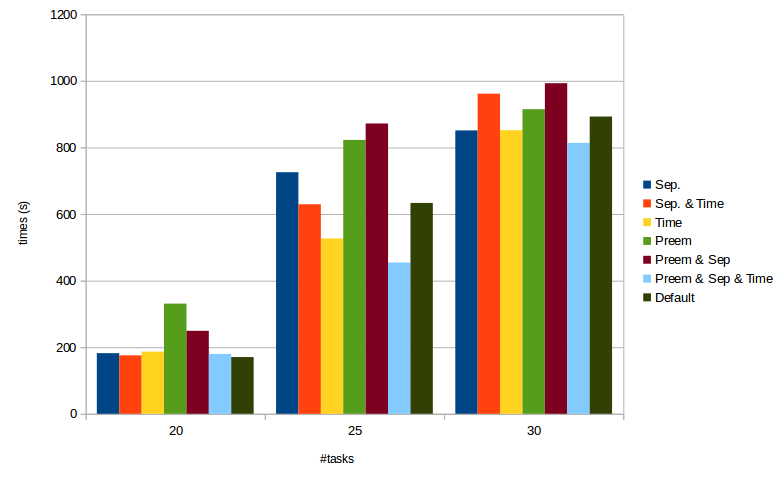
\includegraphics[height=5cm, width=9cm]{time_CECSP.png}
\end{center}
\end{frame}


\begin{frame}
\frametitle{Solved instances comparison for the CECSP}
\begin{itemize}
\item Instances of {\color{gray!50!black!70}\it [Nattaf et al., 2015]}
\item 10 instances of 20, 25 and 30 tasks
\end{itemize}
\vfill
\begin{center}
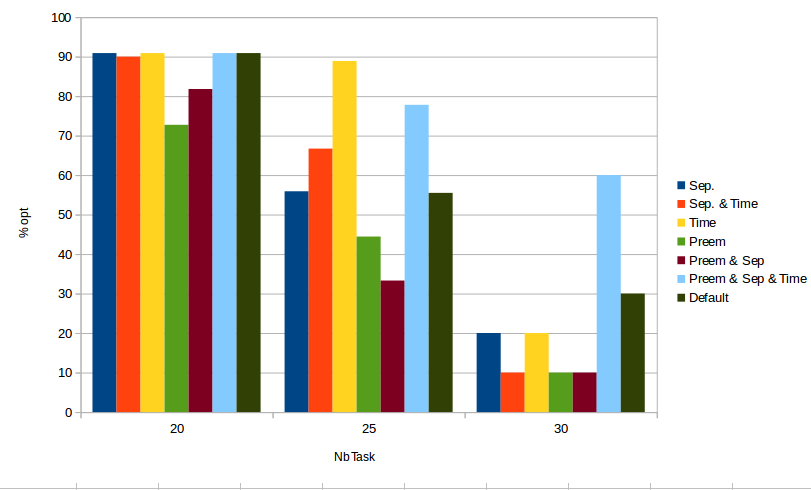
\includegraphics[height=5cm, width=9cm]{opt_CECSP.png}
\end{center}
\end{frame}

\begin{frame}
\frametitle{Time comparison for the RCPSP}
\begin{itemize}
\item Instance of {\color{gray!50!black!70} \it [Koné et al., 2011]}
\item 480 instances of 30 tasks
\end{itemize}
\vfill
\begin{center}
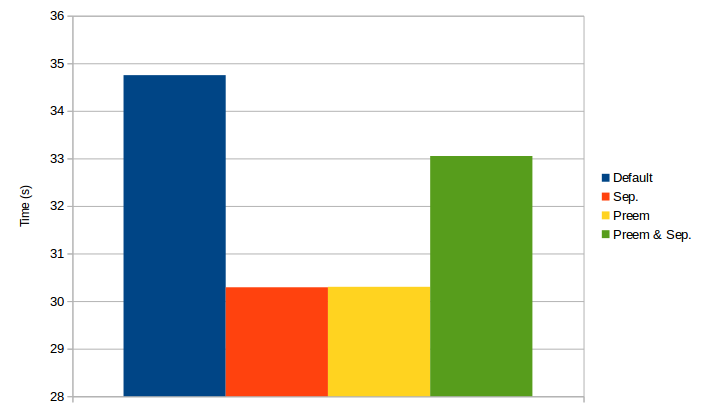
\includegraphics[height=5cm, width=9cm]{timeRCPSP.png}
\end{center}
\end{frame}
